\subsection{问题二的模型的建立和求解}

\subsubsection{具体分析}

针对问题二，本问属于\textbf{标度律建模与多元回归}类问题，需要完成四项递进任务：一是拟合只含参数规模 $N$ 与数据规模 $D$ 的经典标度律；二是对附件 B 的质量信号字段做方向检验，判断其是“质量”还是“难度/噪声”；三是将数据质量 $Q$ 与领域配比 $\bm p$ 纳入经典标度律，建立同时含 $N$、$D$、$Q$、$\bm p$ 的广义标度律\cite{muennighoff2023scaling}；四是分析各因素的边际效用与弹性，推导质量与参数规模相互替代的条件。本问综合采用稳健非线性最小二乘拟合经典 Chinchilla 标度律，采用控制变量组内相关检验判定质量字段方向，采用信息准则与内插外推表现比较四类广义标度律形式，并基于弹性分析与等损失曲线刻画质量—参数替代关系。

首先利用 Pythia 主拟合数据拟合 $L=E+A/N^{\alpha}+B/D^{\beta}$ 形式的经典标度律，并以“小模型训练、大模型留出”的方式检验参数可迁移性；接着在控制 $N$、$D$ 的组内条件下审计 $Q_{\text{score}}$ 与损失的相关方向，据此确定质量定义；然后将 Pythia 与半合成质量数据联合拟合，比较四种质量项形式并择优；最后计算各因素弹性与等损失曲线，给出“提升数据质量等价于增加多少参数量”的替代率，并用问题一的配比系数刻画领域间的替代与互补结构。

\subsubsection{模型准备}

\textbf{1.数据预处理}

本问数据来自附件 B：B1 为 Pythia 系列模型在多个参数规模下的训练损失轨迹（1{,}176 点，8 个模型 $\times$ 147 个检查点）\cite{biderman2023pythia}；B2 为 Cerebras 半合成轨迹；B3 为 8 条 Pythia 插值轨迹（8$\times$500）；B4 为 12 个模型族的跨族收敛点；B5 为已发表标度律数据；B6/B7 为含 $Q_{\text{score}}$ 的半合成质量实验；B8 为大规模矩阵（含外推段）；B9/B10 为百亿参数以上的模型元数据与预估损失。经典标度律以 $N$（参数量，B）与 $D$（训练数据量，B tokens）为自变量、验证损失 $L$ 为因变量；广义标度律进一步引入质量 $Q$。由于 $N$、$D$ 均跨多个数量级，拟合一律在原函数上进行（而非双对数线性化），以保留不可约损失 $E$ 的常数项结构。

\textbf{2.质量字段方向审计}

附件 B 的 $Q_{\text{score}}$ 字段语义未在数据说明中给出，必须先判定方向。判据是：在控制 $N$、$D$ 相同（即同一 $(N,D)$ 分组内）的前提下，若 $Q_{\text{score}}$ 与损失显著正相关，则其为“难度/噪声比例”，须取补变换；若显著负相关，则其本身即为“质量”指标。审计结果如表\ref{tab:p2_dir}所示。

\begin{longtable}{>{\centering\arraybackslash}p{0.18\textwidth}>{\centering\arraybackslash}p{0.10\textwidth}>{\centering\arraybackslash}p{0.12\textwidth}>{\centering\arraybackslash}p{0.16\textwidth}>{\raggedright\arraybackslash}p{0.36\textwidth}}
  \caption{质量字段 $Q_{\text{score}}$ 的方向审计（控制 $N$、$D$ 的组内相关）}
  \label{tab:p2_dir} \\
  \toprule
  数据集 & 样本数 & 分组数 & 组内相关 $r$ & 结论 \\
  \midrule
  \endfirsthead
  \caption{质量字段方向审计（续）} \\
  \toprule
  数据集 & 样本数 & 分组数 & 组内相关 $r$ & 结论 \\
  \midrule
  \endhead
  \bottomrule
  \endfoot
  B6 & 360 & 45 & $-0.925$ & $Q$ 越大损失越低：\textbf{质量指标}（$Q=1$ 为最优） \\
  B7 & 450 & 45 & $-0.918$ & 与 B6 一致，可作独立验证 \\
  B8（校准段） & 984 & 90 & $+0.995$ & 方向与 B6/B7 相反：\textbf{口径不一致} \\
  B8（外推段） & 720 & 60 & $+0.968$ & 同上 \\
\end{longtable}

由表\ref{tab:p2_dir}可知，B6 与 B7 独立地给出 $-0.925$ 与 $-0.918$ 的组内相关，可确认 $Q_{\text{score}}$ 就是数据质量（越高越好），故取 $Q=Q_{\text{score}}$，与问题一“越高越好”的口径一致。但 B8 的两个子集给出相反符号（$+0.995$、$+0.968$），且其最小损失（$0.50$）低于由 Pythia 标定的不可约损失 $E$，说明 B8 与 B6/B7 使用了不同的质量口径（或将质量定义反号），**不能并入拟合**；本文仅在其方向重定向（取 $1-Q_{\text{score}}$）后作一致性检验，并据此明确标注半合成数据的可信度边界。

\textbf{3.算法选择}

本问涉及经典标度律拟合、字段方向检验与广义标度律建模三类任务。经典标度律比较双对数线性回归与非线性最小二乘：前者忽略常数项 $E$ 会引入偏置，故采用带界约束的非线性最小二乘直接拟合原函数，并使用 soft-$L_1$ 稳健损失以降低个别检查点的杠杆效应。方向检验采用控制 $(N,D)$ 的组内相关，可剔除规模与数据量的混杂。广义标度律对四种候选形式做同口径比较，评价指标为联合拟合优度、B6 内部拟合优度、B7 新增点外推相关与 AIC，结果如表\ref{tab:p2_form}所示。

\begin{longtable}{>{\centering\arraybackslash}p{0.28\textwidth}>{\centering\arraybackslash}p{0.13\textwidth}>{\centering\arraybackslash}p{0.13\textwidth}>{\centering\arraybackslash}p{0.13\textwidth}>{\centering\arraybackslash}p{0.10\textwidth}>{\centering\arraybackslash}p{0.13\textwidth}}
  \caption{广义标度律候选形式的比较}
  \label{tab:p2_form} \\
  \toprule
  质量项形式 & 联合 $R^2$ & B6 拟合 $R^2$ & B7 新增点 $r$ & 参数数 & AIC \\
  \midrule
  \endfirsthead
  \caption{广义标度律候选形式的比较（续）} \\
  \toprule
  质量项形式 & 联合 $R^2$ & B6 拟合 $R^2$ & B7 新增点 $r$ & 参数数 & AIC \\
  \midrule
  \endhead
  \bottomrule
  \endfoot
  \textbf{加性质量缺口 $C(1-Q)^{\gamma}$} & \textbf{0.9896} & \textbf{0.9556} & 0.991 & 7 & $\mathbf{-10236}$ \\
  质量同时乘 $N$ 与 $D$ & 0.9882 & 0.9495 & \textbf{0.991} & 7 & $-10042$ \\
  加性质量亏损 $CQ^{-\gamma}$ & 0.9848 & 0.9349 & 0.991 & 7 & $-9660$ \\
  质量作有效数据乘子 & 0.9745 & 0.8905 & 0.983 & 6 & $-8866$ \\
\end{longtable}

如表\ref{tab:p2_form}所示，四类形式的 B7 新增点外推相关均不低于 $0.983$，说明质量效应稳健存在；其中加性质量缺口形式在联合拟合、B6 内部拟合与 AIC 上均最优，故最终采用该形式。

\subsubsection{模型建立}

\textbf{步骤1：经典标度律模型}

以 Chinchilla 标度律为基础，验证损失 $L$ 满足：
\begin{equation}
    L(N,D) = E + \frac{A}{N^{\alpha}} + \frac{B}{D^{\beta}}
\end{equation}
其中 $E$ 为不可约损失（$N,D\to\infty$ 时的极限），$A/\alpha$ 刻画参数规模的边际收益，$B/\beta$ 刻画数据规模的边际收益。该模型隐含“数据质量取参考水平”的基线假设。

\textbf{步骤2：广义标度律模型}

将质量项以“质量缺口”形式引入，得到广义标度律：
\begin{equation}
    L(N,D,Q) = E + \frac{A}{N^{\alpha}} + \frac{B}{D^{\beta}} + C\,(1-Q)^{\gamma},
    \qquad C>0,\ \gamma>0
\end{equation}
该形式满足题设的自然设计要求：当数据质量达到完美（$Q=1$）时质量缺口项自动消失，模型精确退化为经典 Chinchilla 形式，与既有标度律完全兼容；同时其物理含义清晰——**数据质量决定了可达的不可约损失下限**：
\begin{equation}
    \lim_{N,D\to\infty} L(N,D,Q) = E + C\,(1-Q)^{\gamma} \;\ge\; E
\end{equation}
即无论投入多少算力，劣质语料都无法被规模弥补；反之质量越高，损失下限越低。该形式还避开了“加性质量增益 $E-CQ^{\gamma}$”在 $Q\to1$ 时使损失降到 $E-C<0$ 的非物理缺陷。

\textbf{步骤3：边际效用与弹性分析}

在参考点 $(N_0,D_0,Q_0)$ 处，各因素的边际效用为：
\begin{equation}
    \frac{\partial L}{\partial N} = -\alpha A N^{-\alpha-1},\quad
    \frac{\partial L}{\partial D} = -\beta B D^{-\beta-1},\quad
    \frac{\partial L}{\partial Q} = -\gamma C (1-Q)^{\gamma-1}
\end{equation}
对应弹性为：
\begin{equation}
    \varepsilon_N = \frac{\partial L}{\partial N}\frac{N_0}{L_0},\qquad
    \varepsilon_D = \frac{\partial L}{\partial D}\frac{D_0}{L_0},\qquad
    \varepsilon_Q = \frac{\partial L}{\partial Q}\frac{Q_0}{L_0}
\end{equation}

\textbf{步骤4：质量—参数替代条件}

设质量提升 $\mathrm dQ$ 带来的损失下降等于参数增加 $\mathrm dN$ 带来的损失下降，由等损失条件 $\mathrm dL=0$ 得：
\begin{equation}
    \left|\frac{\partial L}{\partial Q}\right|\mathrm dQ = \left|\frac{\partial L}{\partial N}\right|\mathrm dN
    \quad\Longrightarrow\quad
    \frac{\mathrm dN}{\mathrm dQ} = \frac{\gamma C (1-Q)^{\gamma-1}}{\alpha A N^{-\alpha-1}}
    = \frac{\gamma C}{\alpha A}\,(1-Q)^{\gamma-1}N^{\alpha+1}
\end{equation}
该替代率随 $N^{\alpha+1}$ 增长，说明**模型规模越大，参数扩张的边际效用越低，“以质量换规模”越划算**，这正是问题三在算力约束下权衡质量投入与规模投入的核心依据。

\textbf{步骤5：领域间的替代与互补}

线性混合模型下两个训练域 $i$、$j$ 对 13 个验证域损失的效应向量分别为 $\bm a_i,\bm a_j$，定义二者的可替代度为
\begin{equation}
    s_{ij} = \frac{\langle \bm a_i-\bar{\bm a},\ \bm a_j-\bar{\bm a}\rangle}{\|\bm a_i-\bar{\bm a}\|\,\|\bm a_j-\bar{\bm a}\|}
\end{equation}
其中 $\bar{\bm a}$ 为 17 个域的平均效应向量。$s_{ij}\to1$ 表示两域作用方式趋同、可在配比中相互替代；$s_{ij}\to-1$ 表示作用方式相反、构成互补（需搭配使用）。

\subsubsection{模型求解}

\textbf{1.经典标度律拟合与留出验证}

经典标度律在 B1 全量 1{,}176 点上的拟合结果如图\ref{fig:p2_classic}所示，参数估计如下：
\begin{equation}
    L(N,D) = 1.6898 + \frac{0.3540}{N^{0.3400}} + \frac{1.2403}{D^{0.2799}}
\end{equation}
拟合 $R^2 = 0.9999998$、RMSE $=1.5\times10^{-4}$、MAPE $=0.004\%$。以 4 个最小模型训练、预测其余 4 个更大模型，留出 $R^2$ 仍为 $0.9999997$、MAPE $=0.005\%$，说明标度律参数在模型族内部可迁移。

\begin{figure}[ht]
  \centering
  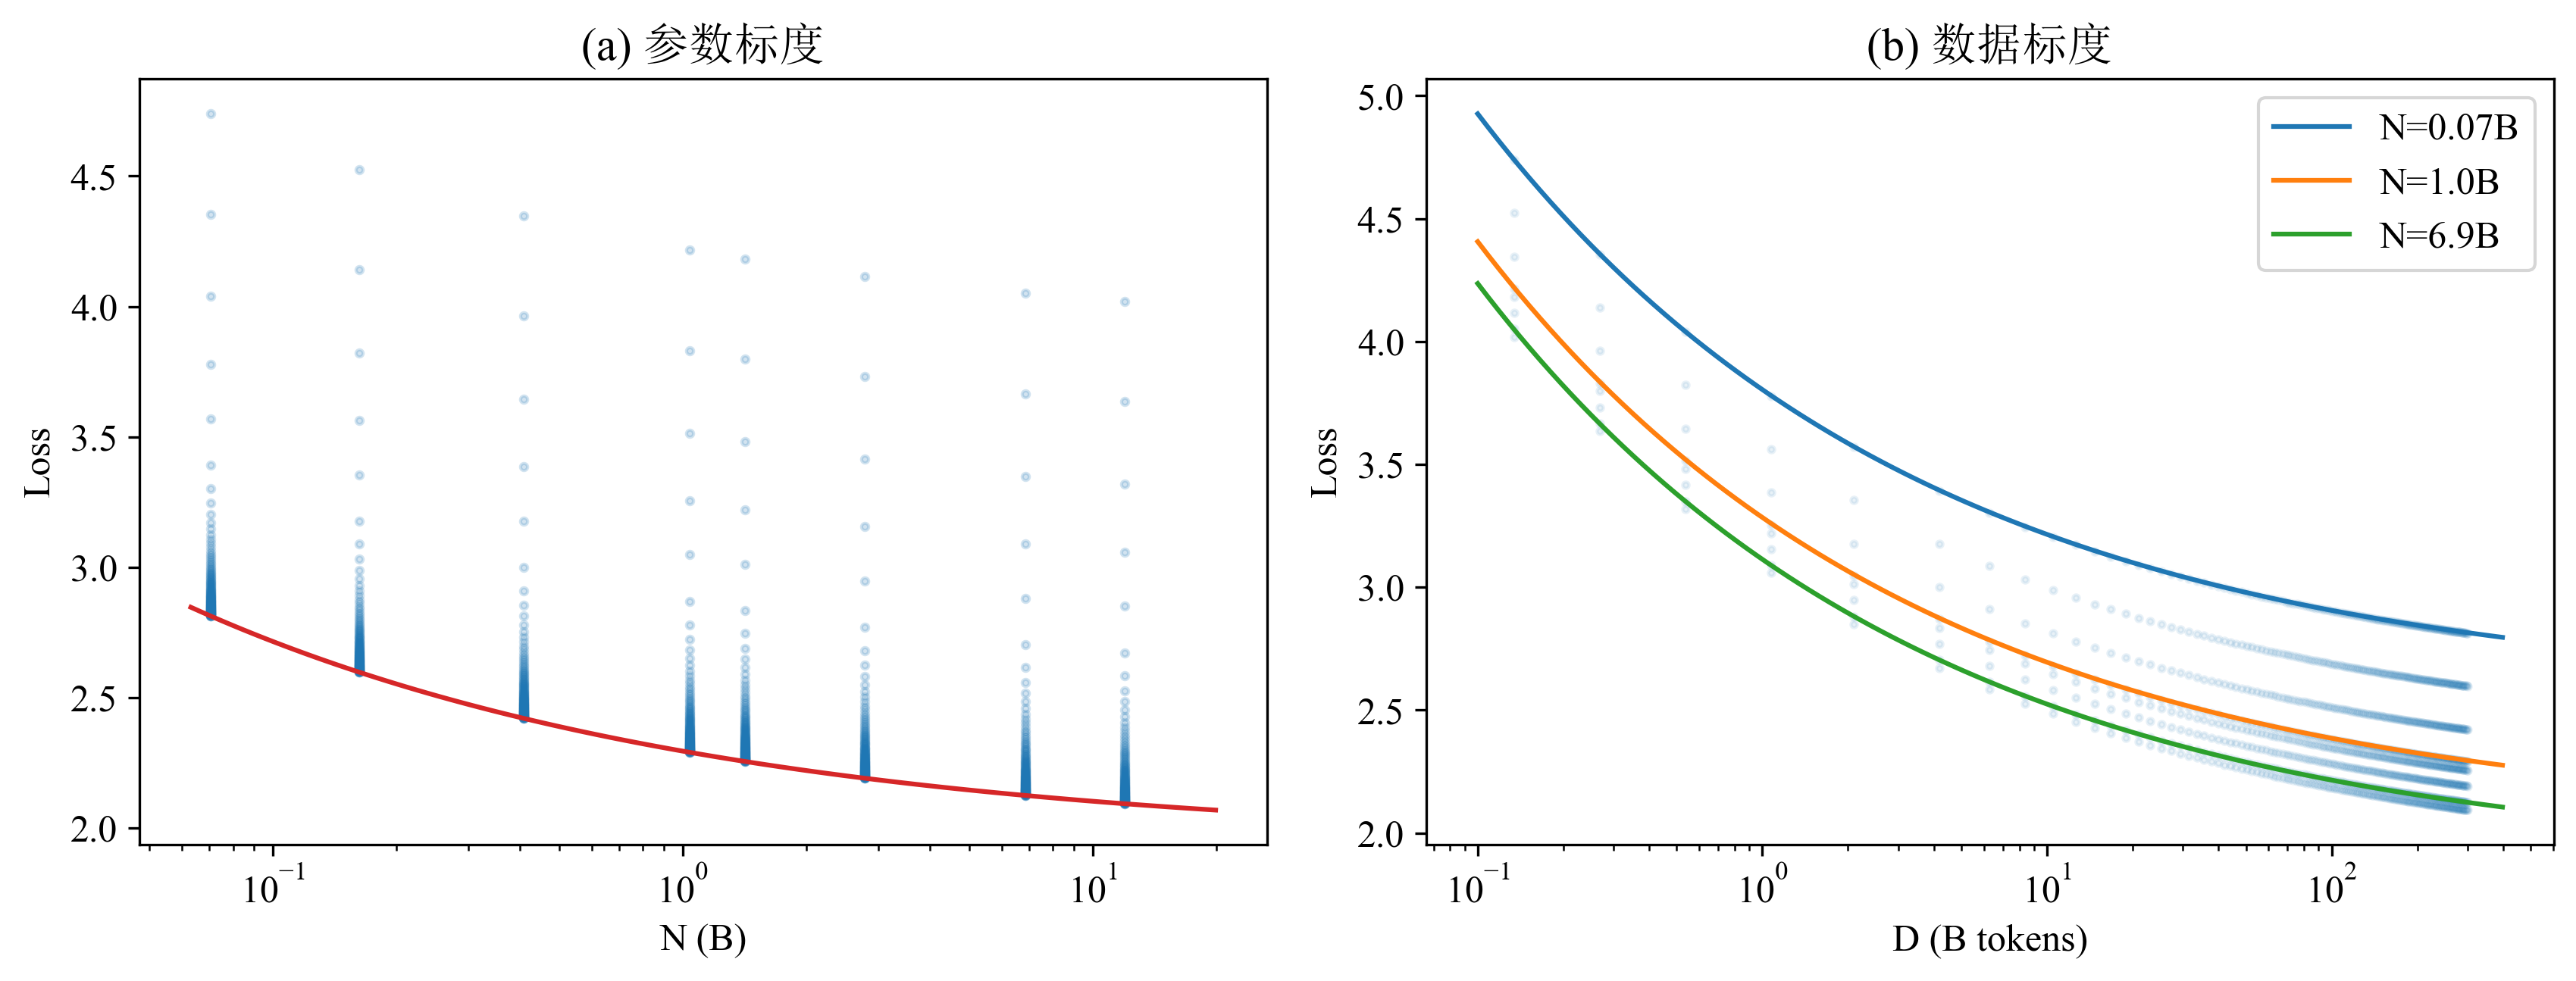
\includegraphics[width=0.92\textwidth]{求解/问题二/图片/图1_经典标度律拟合.png}
  \caption{经典标度律对 Pythia 训练轨迹的拟合（左：随参数规模；右：随数据规模）}
  \label{fig:p2_classic}
\end{figure}

需要客观指出：B1 拟合残差的标准差仅 $1.5\times10^{-4}$，而损失本身的标准差为 $0.342$，即该附件的损失值几乎是 $(N,D)$ 的无噪声函数。因此 B1 上的极高 $R^2$ 只能证明 Chinchilla 函数形式与数据自洽，**不能替代外部验证**；真实泛化能力必须由 B2/B4/B5 等独立来源检验（见本节第 3 部分）。

\textbf{2.广义标度律参数估计}

将 Pythia（无质量信息，取参考质量 $Q=1$）与 B6 质量实验联合拟合，采用表\ref{tab:p2_form}选定的加性质量缺口形式，参数估计如表\ref{tab:p2_params}所示。

\begin{longtable}{>{\centering\arraybackslash}p{0.30\textwidth}>{\centering\arraybackslash}p{0.18\textwidth}>{\centering\arraybackslash}p{0.20\textwidth}>{\raggedright\arraybackslash}p{0.24\textwidth}}
  \caption{广义标度律参数估计}
  \label{tab:p2_params} \\
  \toprule
  参数 & 估计值 & 参数 & 估计值 \\
  \midrule
  \endfirsthead
  \caption{广义标度律参数估计（续）} \\
  \toprule
  参数 & 估计值 & 参数 & 估计值 \\
  \midrule
  \endhead
  \bottomrule
  \endfoot
  不可约损失 $E$ & 1.6558 & 数据规模指数 $\beta$ & 0.2767 \\
  规模系数 $A$ & 0.3808 & 质量缺口系数 $C$ & 0.3544 \\
  规模指数 $\alpha$ & 0.3266 & 质量指数 $\gamma$ & 0.9779 \\
  数据系数 $B$ & 1.2515 & 联合拟合 $R^2$ & 0.9896 \\
\end{longtable}

由表\ref{tab:p2_params}可知，质量指数 $\gamma=0.9779\approx1$，说明质量缺口近似线性地压低损失下限；联合拟合 $R^2=0.9896$、RMSE $=0.036$、MAPE $=0.66\%$，引入质量项后并未牺牲拟合精度。质量缺口对损失的影响如图\ref{fig:p2_quality}所示，质量对损失下限的决定作用可由式 $E+C(1-Q)^{\gamma}$ 直接读出：当 $Q=1$ 时下限为 $1.656$，$Q=0.6$ 时为 $1.802$，$Q=0.3$ 时为 $2.135$。

\begin{figure}[ht]
  \centering
  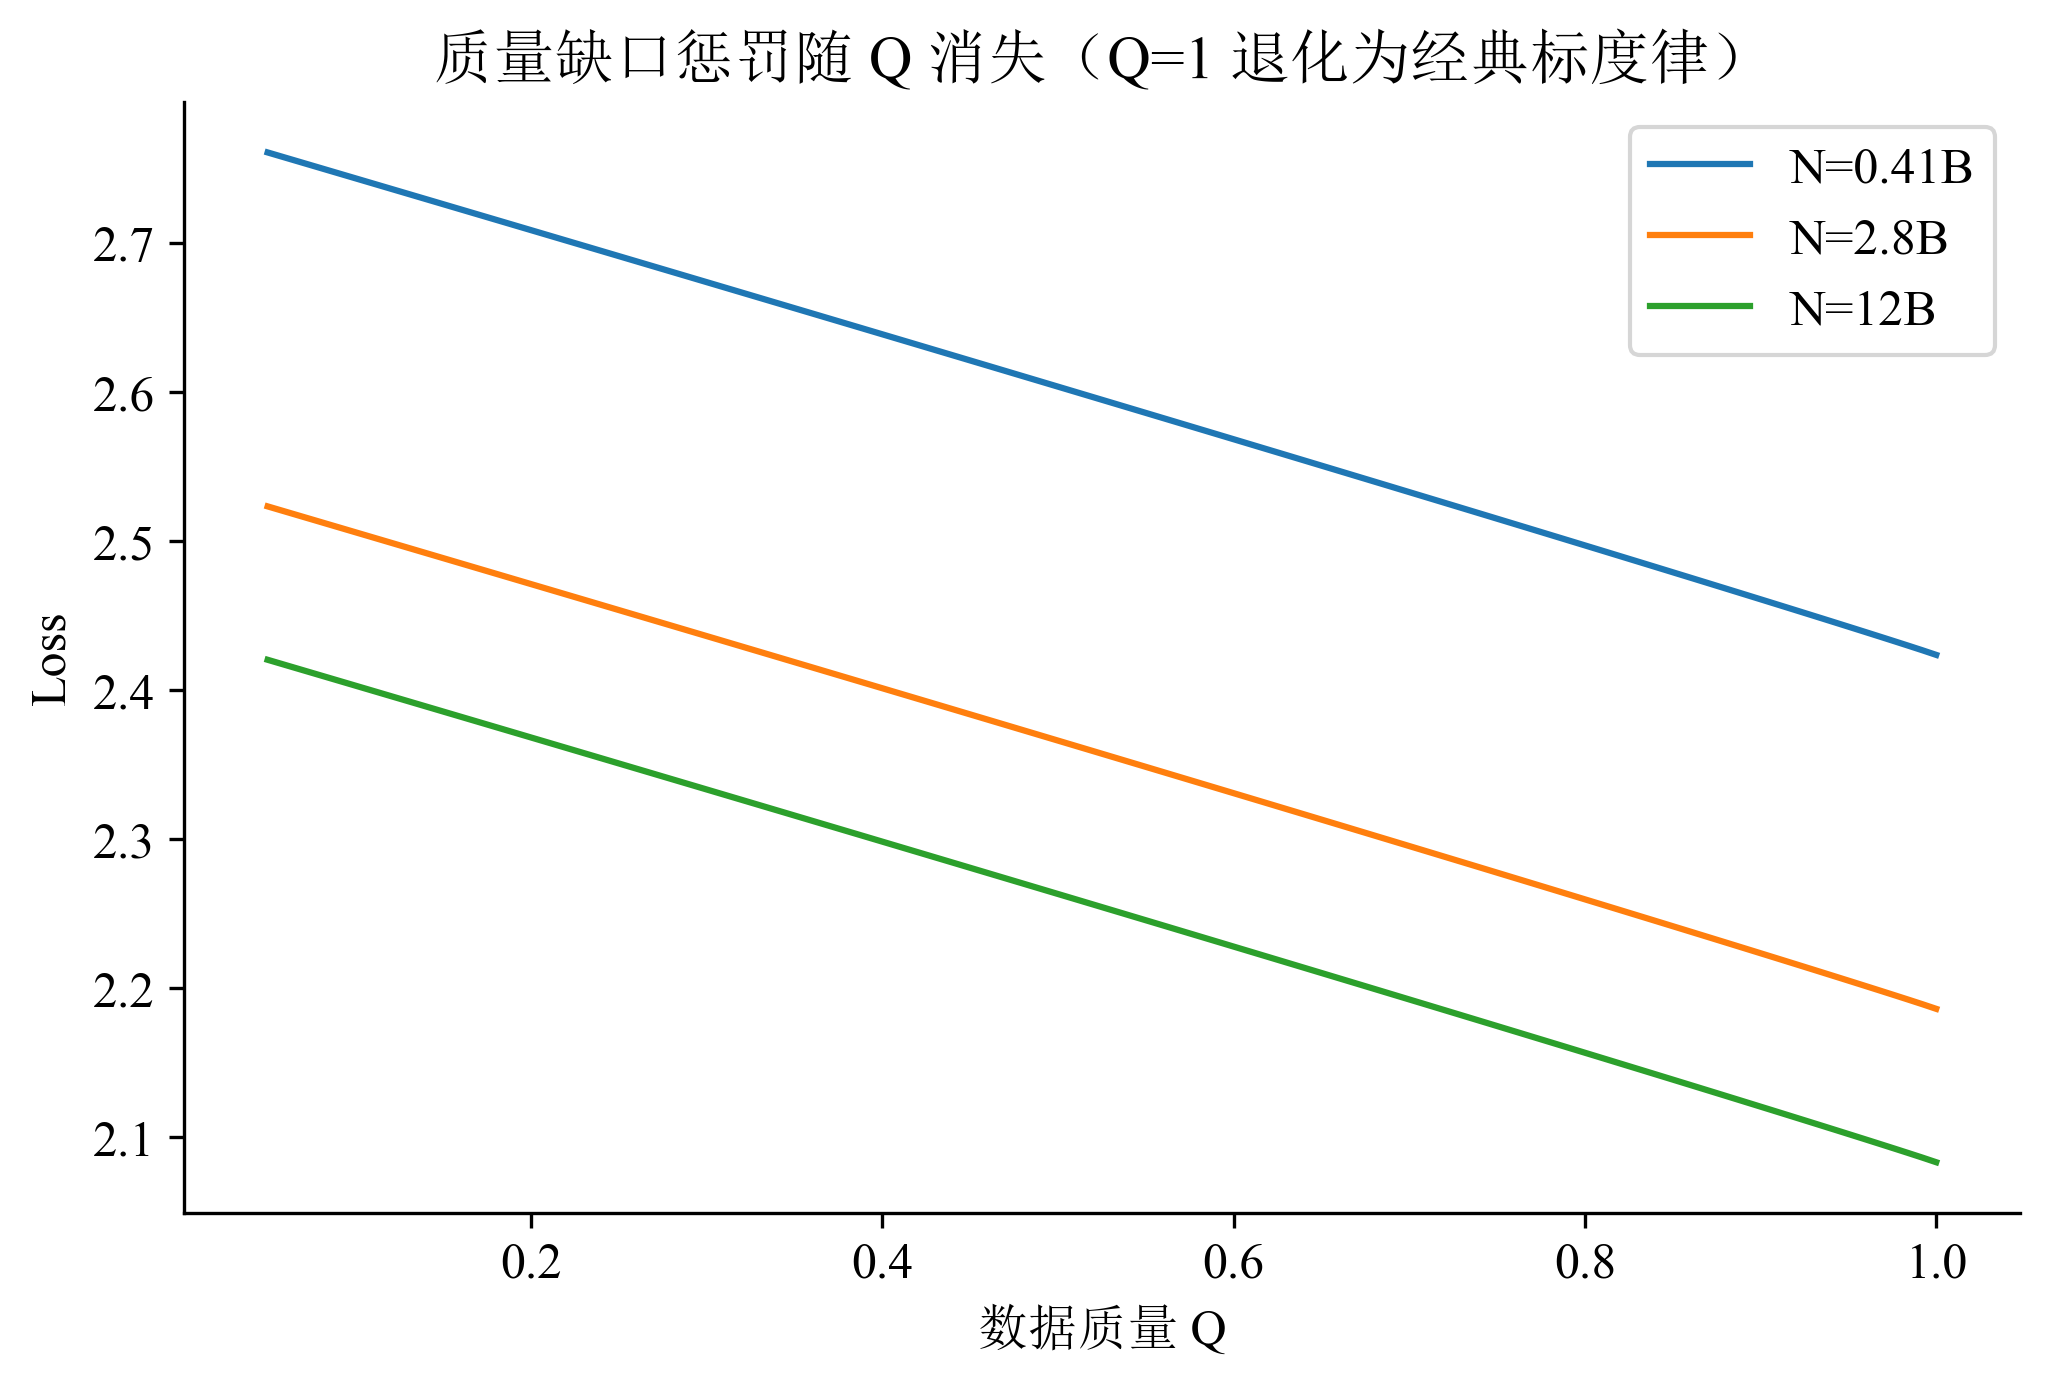
\includegraphics[width=0.62\textwidth]{求解/问题二/图片/图3_质量边际影响.png}
  \caption{固定 $N$、$D$ 时数据质量对损失的决定作用（$Q=1$ 退化为经典标度律）}
  \label{fig:p2_quality}
\end{figure}

\textbf{3.分层验证与稳健性}

广义标度律在 6 个独立来源上的分层验证结果如表\ref{tab:p2_val}所示，预测—实测对比如图\ref{fig:p2_general}所示。

\begin{longtable}{>{\raggedright\arraybackslash}p{0.32\textwidth}>{\centering\arraybackslash}p{0.10\textwidth}>{\centering\arraybackslash}p{0.14\textwidth}>{\centering\arraybackslash}p{0.12\textwidth}>{\centering\arraybackslash}p{0.12\textwidth}>{\centering\arraybackslash}p{0.12\textwidth}}
  \caption{广义标度律的分层验证}
  \label{tab:p2_val} \\
  \toprule
  验证来源 & 样本数 & 性质 & $r$ & RMSE & MAPE(\%) \\
  \midrule
  \endfirsthead
  \caption{广义标度律的分层验证（续）} \\
  \toprule
  验证来源 & 样本数 & 性质 & $r$ & RMSE & MAPE(\%) \\
  \midrule
  \endhead
  \bottomrule
  \endfoot
  B4 跨族收敛点 & 57 & 真实 & 0.975 & 0.293 & 8.8 \\
  B5 已发表标度律 & 44 & 真实 & 0.910 & 0.193 & 8.0 \\
  B7 质量扩展新增点 & 90 & 半合成 & 0.991 & 0.056 & 1.6 \\
  B10 百亿参数以上 & 128 & 估算 & 1.000 & 0.020 & 1.0 \\
  B2 Cerebras 族外 & 1{,}029 & 半合成 & 0.666 & 1.245 & 33.7 \\
  B8 大规模矩阵（方向重定向） & 984 & 半合成 & 0.638 & 1.294 & 133.4 \\
\end{longtable}

\begin{figure}[ht]
  \centering
  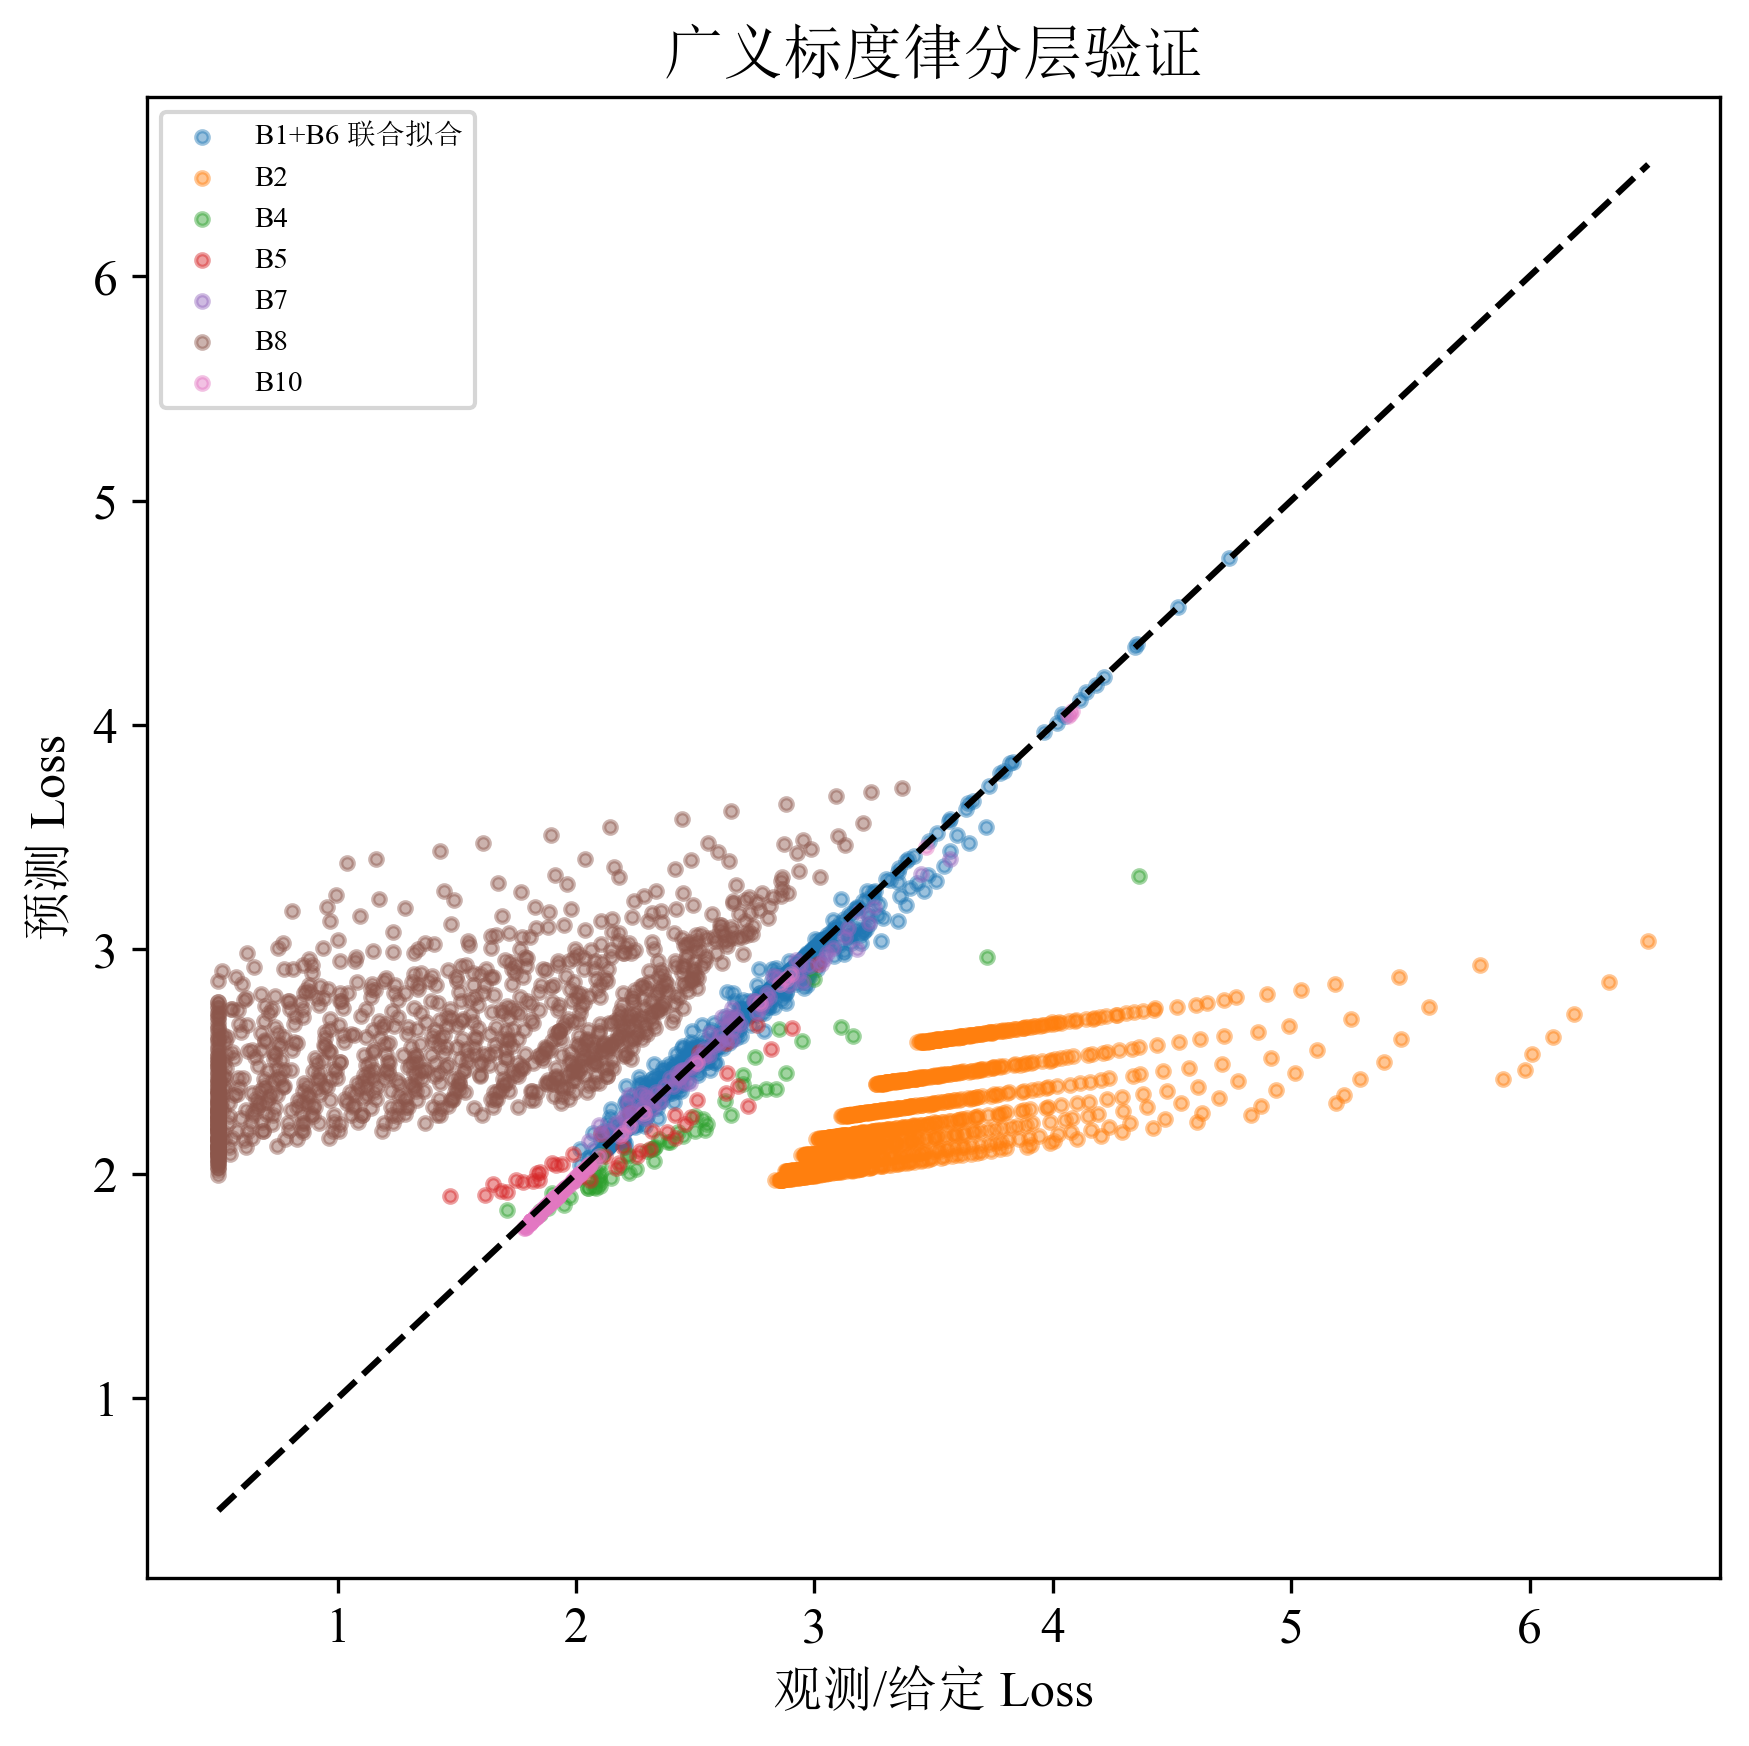
\includegraphics[width=0.62\textwidth]{求解/问题二/图片/图2_广义标度律验证.png}
  \caption{广义标度律预测值与实测损失的多源对比}
  \label{fig:p2_general}
\end{figure}

由表\ref{tab:p2_val}可知：（1）在真实数据上（B4 跨族、B5 文献），模型的相关达 $0.975$ 与 $0.910$、平均相对误差控制在 $8\%$ 量级，说明标度律具备跨族泛化能力；（2）在半合成质量数据上（B7 新增点、B10 估算），相关达 $0.991$ 与 $1.000$，验证了质量项的外推一致性；（3）B2（Cerebras 半合成轨迹）的 MAPE 达 $33.7\%$，说明该半合成数据的校准基线与 Pythia 标度律存在系统性差异，不宜作为定量验证依据；（4）B8 在大规模参数段的最小损失（$0.50$）低于模型不可约损失下限（$1.656$），即使按方向重定向后仍无法拟合（MAPE $133\%$），进一步印证其口径异常。上述分层结论明确界定了本文标度律的可信度边界：**定量结论适用于 $0.07\sim700$B 参数、$5\sim2\times10^4$B tokens 区间的真实与半合成（B6/B7）数据**；B2、B8 仅作定性参考。

此外，用 B3 的 8 条插值轨迹检验数据规模指数：在每条轨迹内（$N$ 固定）以 $L-(E+AN^{-\alpha})$ 对 $D$ 做双对数回归，得到的幂指数为 $-0.2806\sim-0.2803$，与经典拟合的 $-\beta=-0.2799$ 高度一致，说明数据标度关系在训练轨迹内部同样成立。

\textbf{4.弹性、替代关系与领域替代互补}

规模与质量的边际效用对比如图\ref{fig:p2_margin}所示，等损失曲线如图\ref{fig:p2_subst}所示，弹性与替代率计算结果如表\ref{tab:p2_subst}所示。

\begin{figure}[ht]
  \centering
  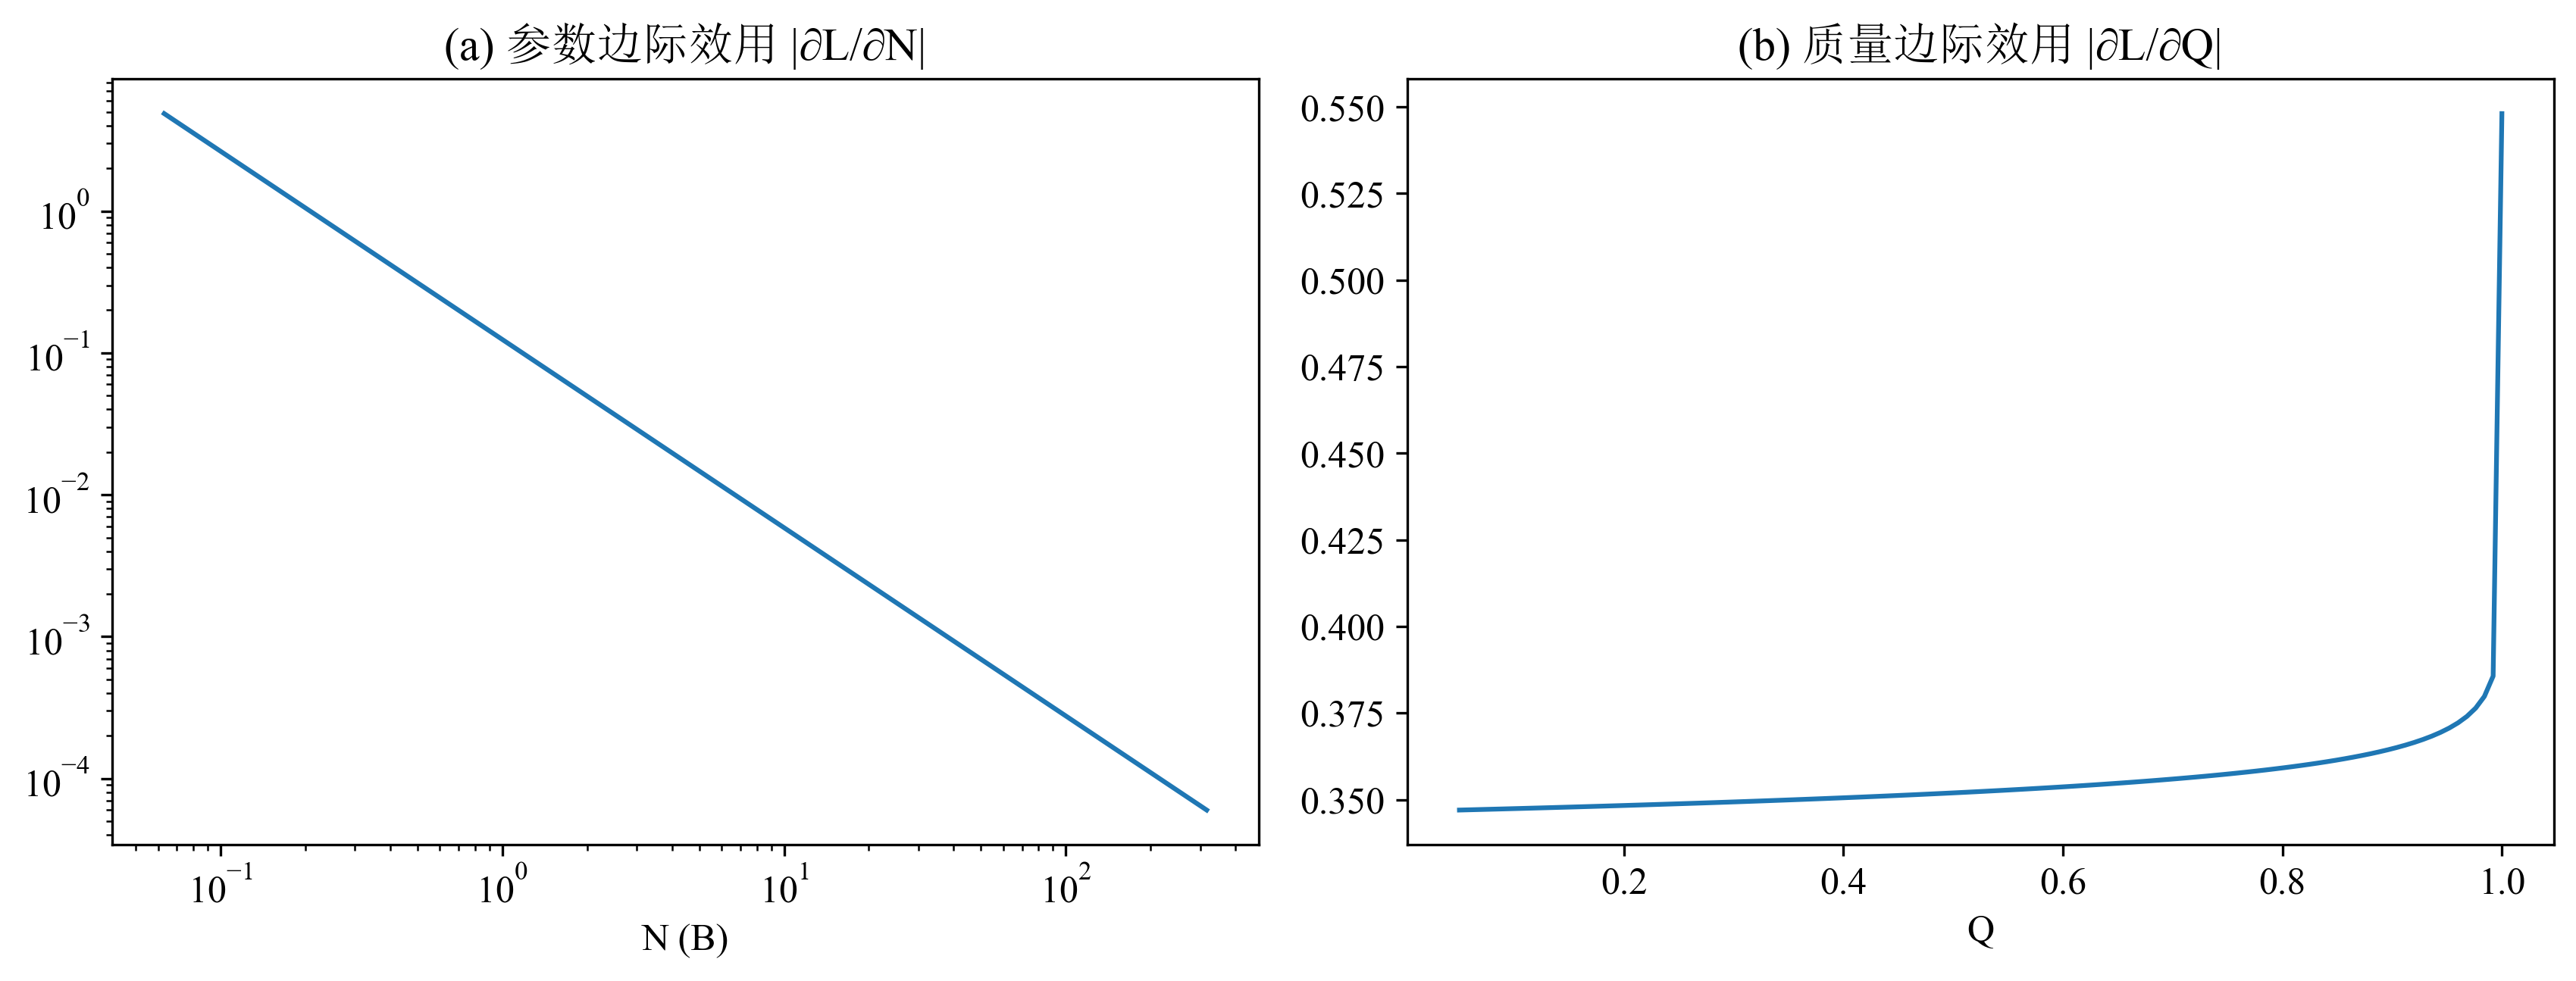
\includegraphics[width=0.92\textwidth]{求解/问题二/图片/图4_边际效用对比.png}
  \caption{规模边际效用与质量边际效用的对比（左：随 $N$ 衰减；右：随 $Q$ 递减）}
  \label{fig:p2_margin}
\end{figure}

\begin{figure}[ht]
  \centering
  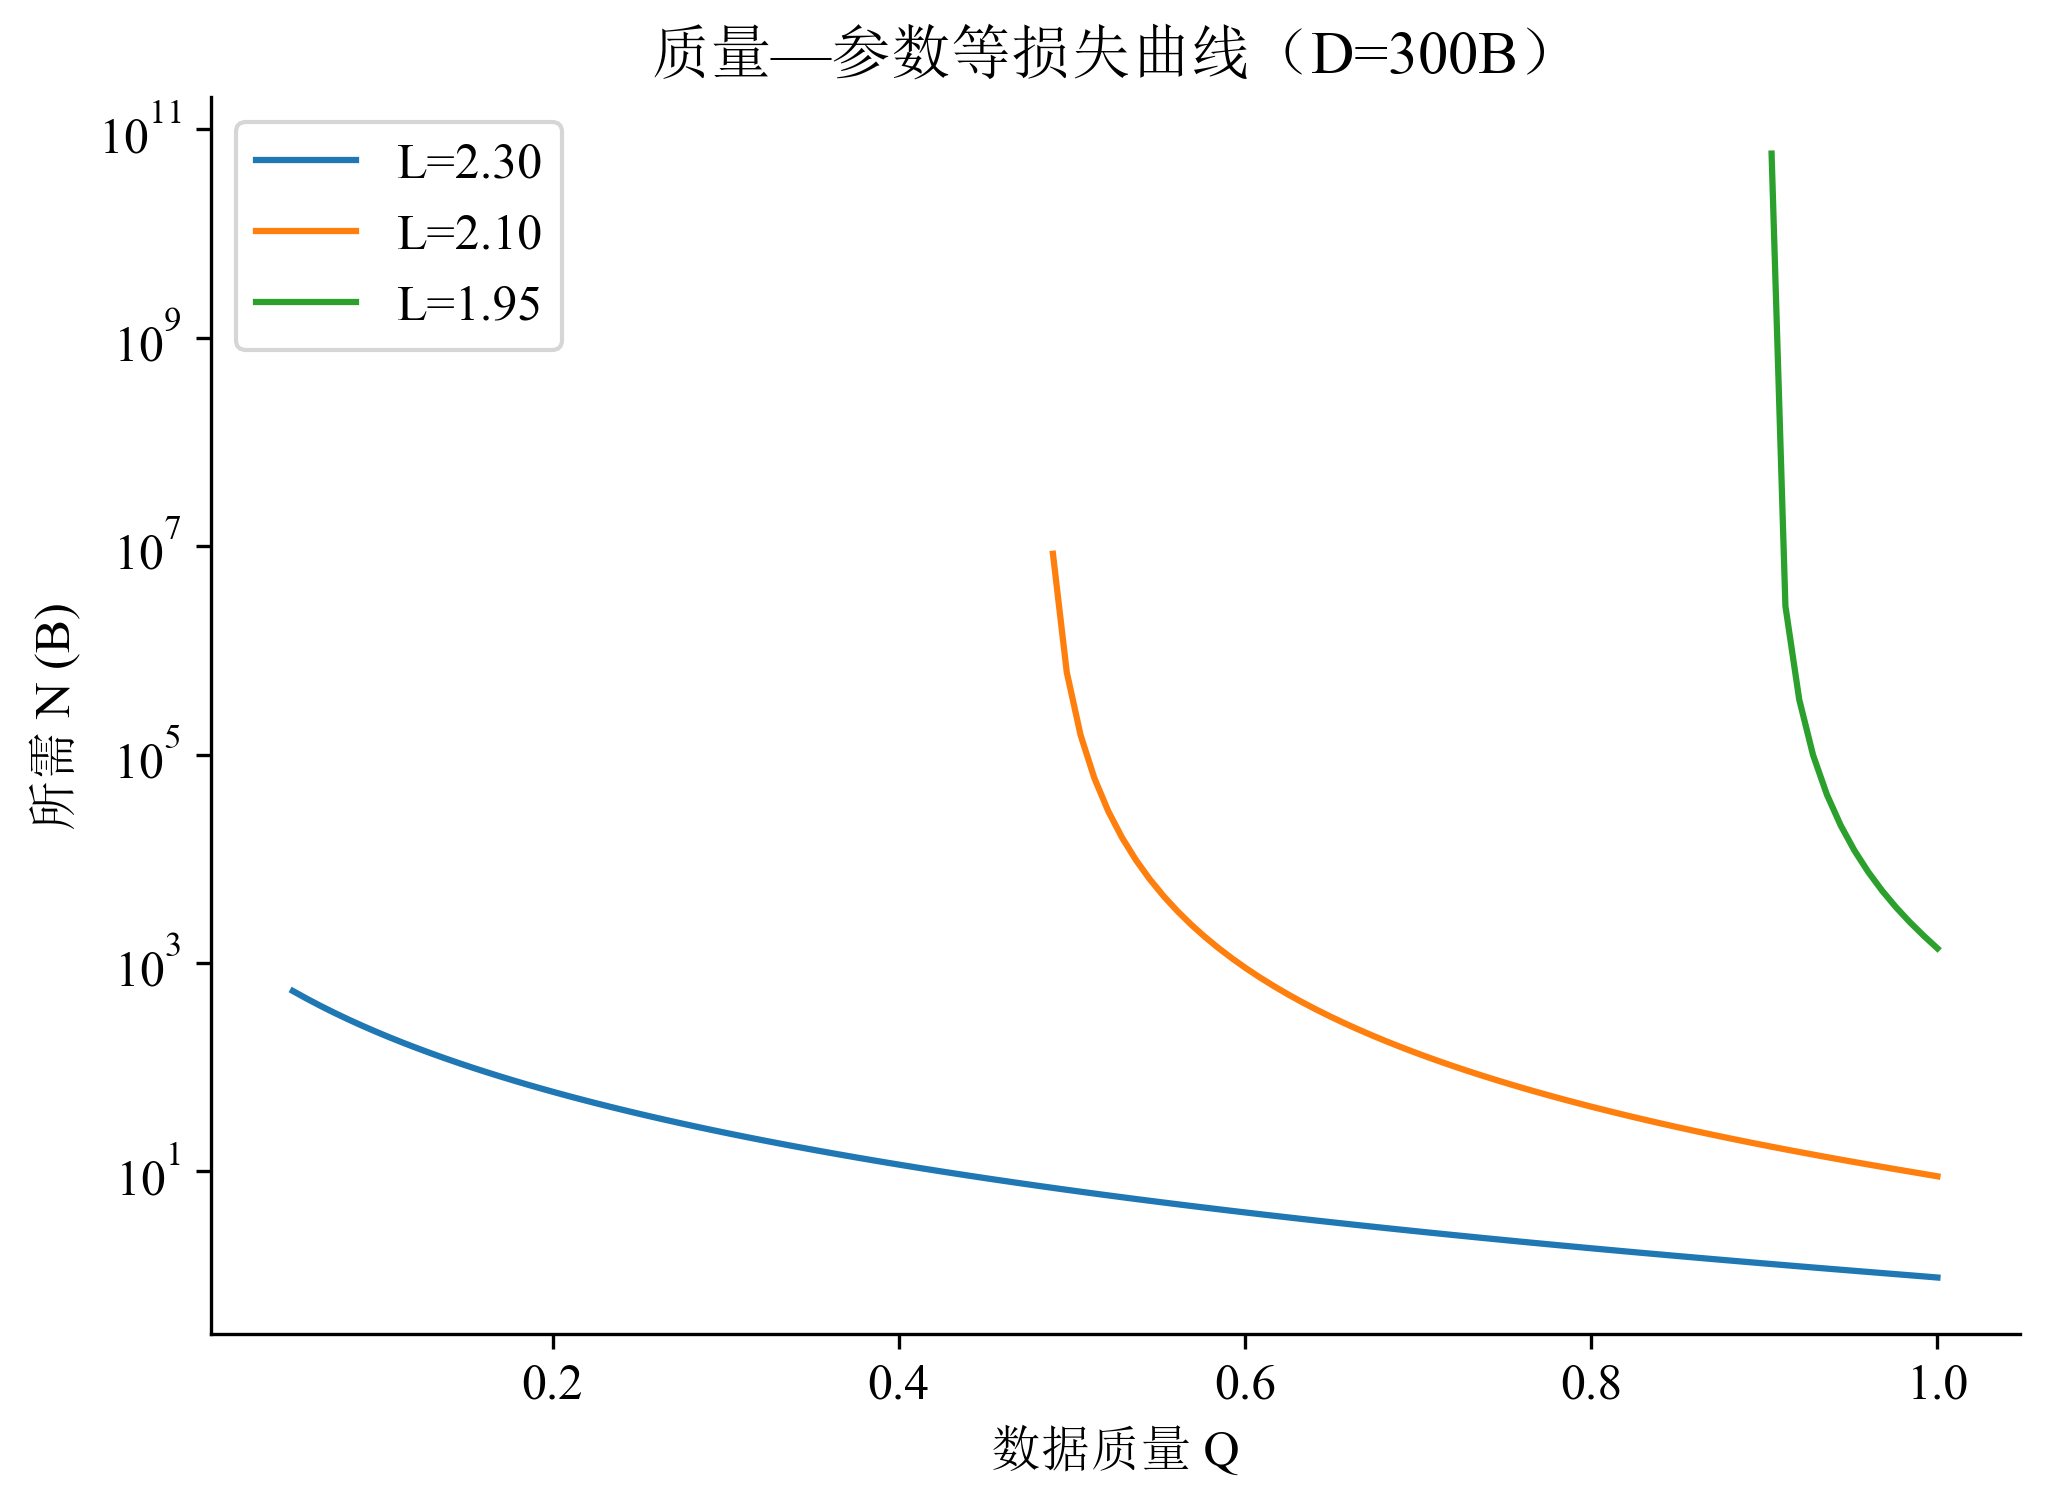
\includegraphics[width=0.60\textwidth]{求解/问题二/图片/图5_质量参数替代.png}
  \caption{等损失曲线：达到同一损失所需参数量随质量的演化（$D=300$B）}
  \label{fig:p2_subst}
\end{figure}

\begin{longtable}{>{\centering\arraybackslash}p{0.13\textwidth}>{\centering\arraybackslash}p{0.11\textwidth}>{\centering\arraybackslash}p{0.10\textwidth}>{\centering\arraybackslash}p{0.13\textwidth}>{\centering\arraybackslash}p{0.13\textwidth}>{\centering\arraybackslash}p{0.13\textwidth}>{\raggedright\arraybackslash}p{0.20\textwidth}}
  \caption{弹性与质量—参数替代关系}
  \label{tab:p2_subst} \\
  \toprule
  $N_0$(B) & $D_0$(B) & $Q_0$ & $\varepsilon_N$ & $\varepsilon_D$ & $\varepsilon_Q$ & $\mathrm dN/\mathrm dQ$ (B/单位) \\
  \midrule
  \endfirsthead
  \caption{弹性与质量—参数替代关系（续）} \\
  \toprule
  $N_0$(B) & $D_0$(B) & $Q_0$ & $\varepsilon_N$ & $\varepsilon_D$ & $\varepsilon_Q$ & $\mathrm dN/\mathrm dQ$ (B/单位) \\
  \midrule
  \endhead
  \bottomrule
  \endfoot
  1 & 100 & 0.6 & $-0.0491$ & $-0.0383$ & $-0.0838$ & 2.844 \\
  12 & 300 & 0.6 & $-0.0248$ & $-0.0321$ & $-0.0953$ & 76.838 \\
\end{longtable}

由表\ref{tab:p2_subst}可知：（1）在 $N_0=1$B、$D_0=100$B、$Q_0=0.6$ 处，质量弹性 $|\varepsilon_Q|=0.0838$ 约为规模弹性 $|\varepsilon_N|=0.0491$ 的 $1.7$ 倍，即在同等比例投入下质量提升对损失的压制更强；（2）替代率 $\mathrm dN/\mathrm dQ=2.844$ B/单位质量，即数据质量提升 $0.1$ 所带来的损失下降等价于参数量增加约 $0.28$B；（3）替代率随 $N$ 迅速增大（在 $N_0=12$B 处达 $76.8$ B/单位，$0.1$ 的质量提升等价于约 $7.68$B 参数），验证了式 $\mathrm dN/\mathrm dQ\propto N^{\alpha+1}$ 的结论——**规模越大，以质量换规模越划算**。图\ref{fig:p2_subst}的等损失曲线进一步显示，随着质量提高，达到同一损失所需参数量指数级下降。

领域间的替代与互补结构如图\ref{fig:p2_dom}所示。

\begin{figure}[ht]
  \centering
  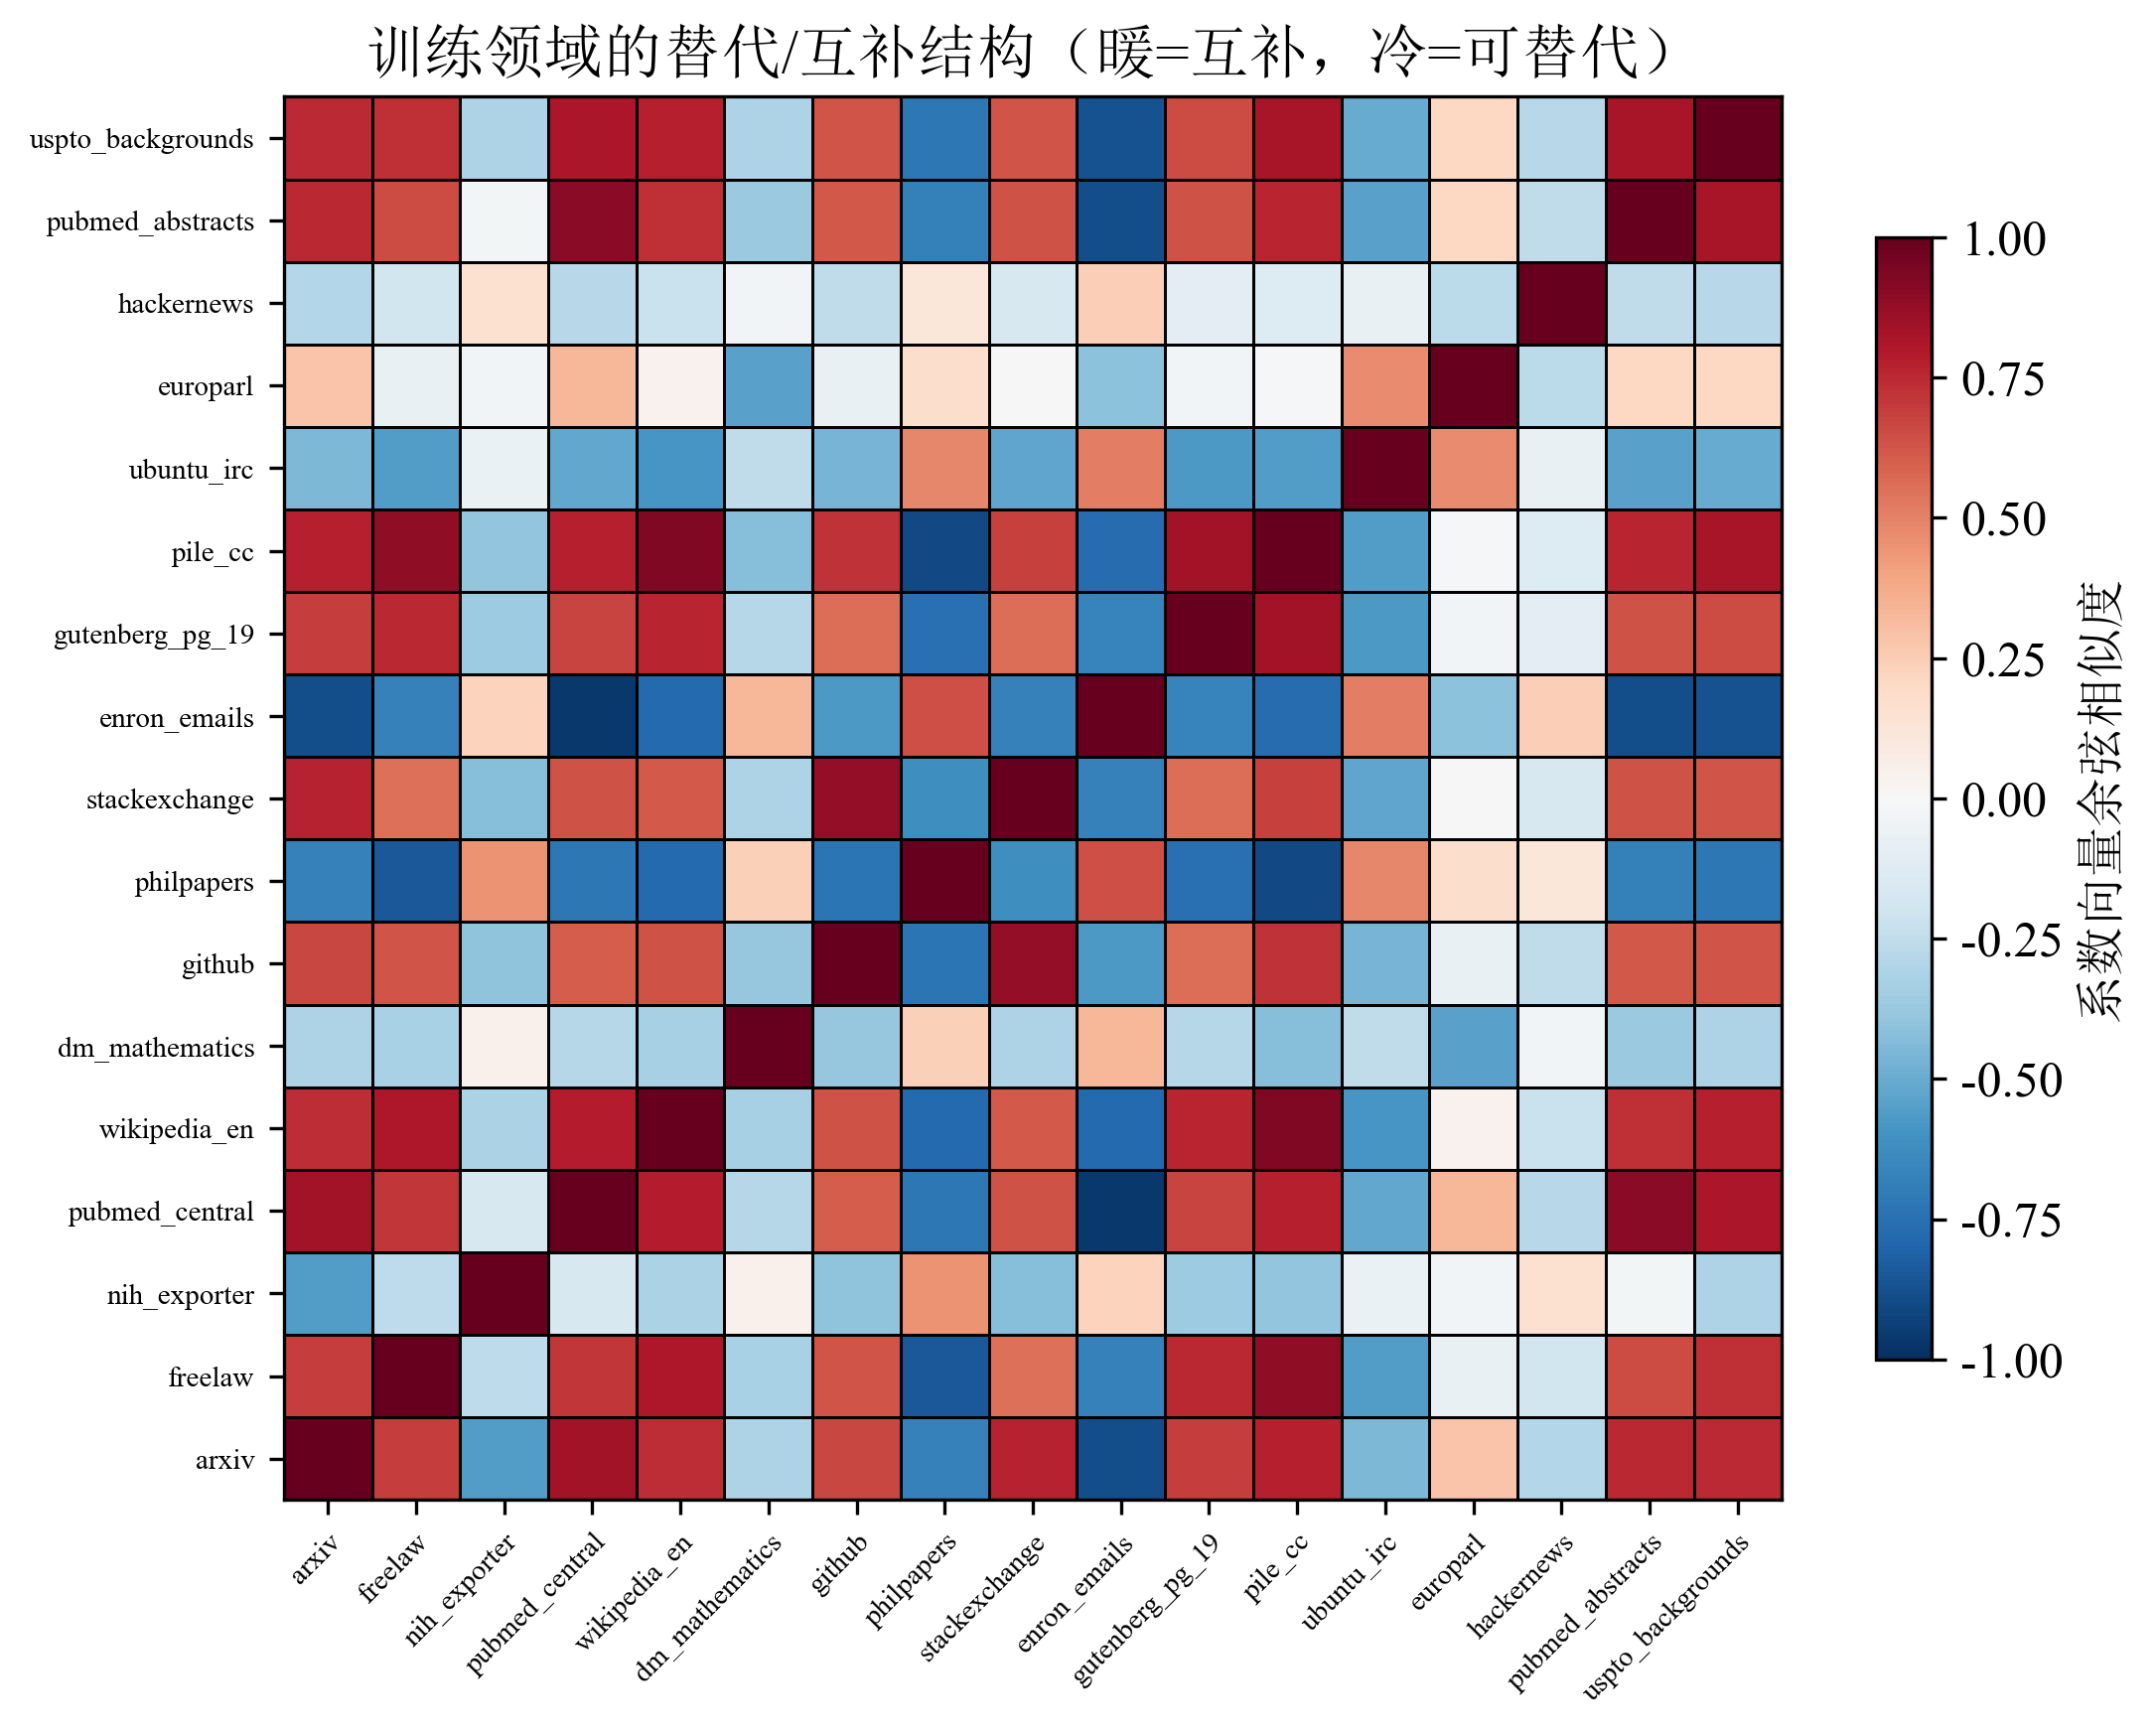
\includegraphics[width=0.62\textwidth]{求解/问题二/图片/图6_领域替代互补.png}
  \caption{训练领域的替代/互补结构（系数向量余弦相似度，暖=互补、冷=可替代）}
  \label{fig:p2_dom}
\end{figure}

由图\ref{fig:p2_dom}可知，（wikipedia\_en, pile\_cc）与（pubmed\_central, pubmed\_abstracts）的相似度最高（$0.925$、$0.903$），即它们对 13 个验证域的作用方式趋同，在配比中互为替代品；而（pubmed\_central, enron\_emails）的相似度为 $-0.967$、作用方式相反，构成互补对。这一结构解释了问题一推荐配比中“学术类域同时上升、网页类域同时下降”的成组变动现象：优化算法实际是在同一替代族内重新分配权重，而非逐域独立调整。

最后，将问题一的推荐配比作为配比项 $M(\bm p)$ 引入广义标度律（$M=\hat L(\bm p_{\text{rec}})-\hat L(\bm p_{\text{ref}})=-0.1988$，即在同等算力下损失下降 $0.199$），说明领域配比虽不增加算力总开销，却能改变算力的使用效率；该修正项将在问题三中作为损失函数的水平平移参与优化。

综合以上结果，本节完成了问题二的求解，得到广义标度律 $L(N,D,Q)$、质量与规模的替代条件以及领域替代互补结构，为问题三提供优化目标。
